
\chapter{Diagonalización de matrices  $\divideontimes$}	


	

\section{Valores y vectores prropios}

Los conceptos de valores y vectores propios cuestan un poco de entender, veamos su definición.

\begin{defi}
Los \textbf{`vectores propios o autovectores'} son los vectores no nulos de una aplicación lineal que, cuando son transformados por ella, dan lugar a un múltiplo escalar de ellos (no cambian de dirección). Este escalar el el \textbf{`valor propio o autovalor'}:

\vspace{4mm}\centerline{\colorbox{LightYellow}{$\boldsymbol{\; A\; \vec v = \lambda \; \vec v  \;,}$}}

\justify
donde $A$ es la matriz de la aplicación lineal, $\vec v$ es el vector propio y $\lambda$ el valor propio o característico. Hay quien usa la raíz alemana y habla de `eigen-valores' y `eigen-vectores'.

\end{defi}

Para el cálculo de los valores y vectores propios de una matriz (aplicación lineal) se sigue el siguiente \emph{`algoritmo'}:

\begin{enumerate}
\item Calcular la `ecuación característica': $\quad det(A-\lambda I)$
\item Encontrar las raíces del `polinomio característico' obtenido: 

$ det(A-\lambda I)=0 \longrightarrow \lambda_i$. Estos son los valores propios.

\item Calcular el vector propio correspondiente a cada uno de los valores propios obtenidos en el paso anterior:	

$A\vec v=\lambda \vec v \to (A-\lambda  I)\vec v=\vec 0$
\end{enumerate}

Para el cálculo de los valores y vectores propios de una matriz también es conveniente tener en cuenta los siguientes `trucos' \textcolor{gris}{(proposiciones que no vamos a demostrar)}.

\begin{itemize}
\item La traza de una matriz A (suma de los elementos de su diagonal principal)	coincide con la suma de los autovalores o valores propios:

$\displaystyle tr(A)=\textcolor{gris}{\sum_{i=1}^n a_{ii}}=\sum_{i=1}^n \lambda_i$

\item El producto de todos los valores propios coincide con el determinante de la matriz.

$\displaystyle det(A)=\prod_{i=1}^n \lambda_i$

\item Si hay una combinación lineal en filas o columnas de $A$, entonces un valor propio, al menos, de la matriz es cero.
\end{itemize}

\begin{ejem}
Dada $A=\left( \begin{matrix} 1&0\\5&2 \end{matrix} \right)$, encuentra sus autovalores y autovectores.

$det(A-\lambda I)=\left| \begin{matrix} 1-\lambda&0\\5&2-\lambda \end{matrix} \right|=\lambda^2-3\lambda+2=0 \longrightarrow \lambda =1 \; \wedge \; \lambda=2$

--- $\lambda =1 \longrightarrow (A-\lambda I)\vec v=\vec 0 \to (A-I)\vec v=\vec 0\to (A-I)\left( \begin{matrix} x\\y \end{matrix} \right) = \left( \begin{matrix} 0\\0 \end{matrix} \right)$ 

\noindent \small{$\left( \begin{matrix} 0&0\\5&1 \end{matrix} \right)\left( \begin{matrix} x\\y \end{matrix} \right) = \left( \begin{matrix} 0\\0 \end{matrix} \right) \to \begin{cases} 0x+0y=0\\5x+y=0 \end{cases} \to y=-5x \Rightarrow (x=1)\; 
\vec v=\left( \begin{matrix} 1\\-5 \end{matrix} \right)$}\normalsize{.}


--- $\lambda =2 \longrightarrow (A-\lambda I)\vec v=\vec 0 \to (A-2I)\vec v=\vec 0\to (A-2I)\left( \begin{matrix} x\\y \end{matrix} \right) = \left( \begin{matrix} 0\\0 \end{matrix} \right)$	

\noindent \small{ $\left( \begin{matrix} -1&0\\5&0 \end{matrix} \right)\left( \begin{matrix} x\\y \end{matrix} \right) = \left( \begin{matrix} 0\\0 \end{matrix} \right) \to \begin{cases} -x+0y=0\\5x+0y=0 \end{cases} \to x=0 \Rightarrow (y=1)\; 
\vec v=\left( \begin{matrix} 0\\1 \end{matrix} \right)$}\normalsize{.}

Conclusión, los valores propios y sus correspondientes valores propios de la matriz A son:

$\lambda=1 \leftrightarrow \vec v=\left( \begin{matrix} 1\\-5 \end{matrix} \right)
\quad; \qquad \qquad  
\lambda = 2 \leftrightarrow \vec v=\left( \begin{matrix} 0\\1 \end{matrix} \right)$
\end{ejem}


\section{Diagonalización de matrices}

\begin{defi}
Una \textbf{matriz diagonalizable} es una matriz cuadrada que se puede transformar en una matriz diagonal.	

La diagonalización de las matrices es del siguiente modo:

\vspace{4mm} \centerline{\colorbox{LightYellow}{$\boxed{ \; \boldsymbol{A=PDP^{-1} \quad \leftrightarrow \quad D=P^{-1}AP}\; }$ ,}}

\justify

donde $A$ es la matriz a diagonalizar, $P$ es la matriz formada por los vectores propios de $A$ escritos como columnas, $P^{-1}$ es la matriz inversa de $P$ y $D$ es la matriz diagonalizada, cuyos elementos de la diagonal principal son los autovalores de $A$. \textcolor{gris}{La matriz $P$ actúa como una matriz de cambio de base, por lo que, en realidad, con esta fórmula estamos cambiando la matriz $A$ a una nueva base en que se convierte en diagonal $D$. Evidentemente, $P$ es una matriz regular o invertible.} 
\end{defi}

No todas las matrices son diagonalizables, tan solo se pueden diagonalizar las matrices que cumplen con unas ciertas características. Se puede saber si una matriz es diagonalizable de distintas maneras:

\begin{itemize}

\item Una matriz cuadrada de orden $n$ es diagonalizable si tiene $n$ vectores propios (o autovectores) linealmente independientes, o dicho de otra forma, si estos vectores forman una base. Eso es debido a que la matriz $P$, que sirve para diagonalizar la matriz dada $A$, está formada por los vectores propios de dicha matriz $A$. Para saber si los autovectores son LI, basta con que el determinante de la matriz $P$ sea diferente de $0$, cosa que significa que la matriz es de rango máximo. $\quad$ \emph{Si $det(P)\neq 0 \to $ matriz diagonalizable.}
\item Una propiedad de los valores y vectores propios es que los autovectores de autovalores diferentes son linealmente independientes. Por lo tanto, si todos los autovalores de la matriz son únicos (todos tienen multiplicidad uno)  la matriz es diagonalizable.
\item Finalmente, existe un teorema, el \emph{`teorema espectral'}, que garantiza la diagonalización de las matrices simétricas con números reales. Es decir, \emph{toda matriz real y simétrica es diagonalizable}.
	
\end{itemize}

Para diagonalizar  una matriz (aplicación lineal) $A$ se sigue el siguiente \emph{`algoritmo'}:

\begin{enumerate}
\item Obtener los valores ($\lambda_i$)y vectores propios ($\vec v_i$) de $A$
\item Construir la matriz $P$ formada los los vectores-columna propios de $A$
\item Verificar que $A$ es digonalizable, está en alguno de los supuestos anteriores.
\item Construir la matriz $D$ en que todos sus elementos son cero excepto los de la diagonal principal, que son los valores propios de $A$:

$D=(d_{ij})=\begin{cases} \lambda_i & \text{ si } i=j \\
0 & \text{ si } i \neq j \end{cases}$	
\end{enumerate}

NOTA: Los vectores propios en $P$ se pueden escribir en cualquier orden, pero entonces, hay que respetar ese mismo orden al escribir los valores propios en $D$: 

$P=\left( \vec v_1 \; | \; \vec v_2 \; | \; \cdots \; | \; \vec v_n \right) \longrightarrow D=\left( \begin{matrix} \lambda_1 &0&\cdots &0 \\ 0&\lambda_2&\cdots & 0 \\ \vdots & \vdots & \ddots & \vdots \\ 0&0&\cdots & \lambda_n \end{matrix} \right)$

\begin{teor}{Aplicaciones de las matrices diagonalizables}
Al estar las matrices diagonales llenas de ceros el cálculo se simplifica muchísimo. Un ejemplo claro de ellos son las `potencias' de las matrices cuadradas:

\vspace{4mm} \centerline{\colorbox{LightYellow}{$\; A^k=PD^kP^{-1} \; , \qquad D^k=diag(\lambda_1^k, \lambda_2^k, \cdots, \lambda_n^k)\; $	}}
\end{teor}
\begin{proofw}

\textcolor{gris}{\noindent $A^2=A\cdot A = (PDP^{-1})\cdot  (PDP^{-1})= PD\; P^{-1} P\; DP^{-1}=  PDIDP^{-1}=PD^2P$}

\noindent \textcolor{gris}{\noindent $A^3=A^2\cdot A= (PD^2P^{-1})\cdot (PDP^{-1})=PD^2\;P^{-1})P\; DP^{-1}=PD^2IDP^{-1}=PD^3P$}

\noindent \textcolor{gris}{\noindent . . . . . . . . . . . . . . . .}

\noindent \textcolor{gris}{\noindent Conjeturamos: $A^k=PD^kP$, necesitaría de una demostración por inducción que de le deja al lector.}
	
\end{proofw}
	



\begin{ejem}
Diagonaliza la matriz $A=\left( \begin{matrix} 2&2\\1&3 \end{matrix} \right)$

$|A-\lambda I|=\left| \begin{matrix} 2-\lambda&2\\1&3-\lambda \end{matrix}  \right|=\lambda^2-5\lambda +4=0 \leftrightarrow \lambda_1=1; \; \wedge \; \lambda_2=4	$

--- $ \lambda=1 \to (A-I)\vec v= \vec 0 \to \left( \begin{matrix} 1&2\\1&2 \end{matrix} \right)\; \left( \begin{matrix} x\\y \end{matrix} \right)=
\left( \begin{matrix} 0\\0 \end{matrix} \right)$

$\begin{cases} x+2y=0\\x+2y=0 \end{cases} \to x=-2y \Rightarrow \vec v_1=\left( \begin{matrix} -2\\1 \end{matrix} \right)$

--- $ \lambda=4 \to (A-4I)\vec v= \vec 0 \to \left( \begin{matrix} -2&2\\1&-1 \end{matrix} \right)\; \left( \begin{matrix} x\\y \end{matrix} \right)=
\left( \begin{matrix} 0\\0 \end{matrix} \right)$

$\begin{cases} -x+2y=0\\x-y=0 \end{cases} \to x=y \Rightarrow \vec v_2=\left( \begin{matrix} 1\\1 \end{matrix} \right)$

Por lo que: $\quad P=\left( \begin{matrix} -2&1\\1&1 \end{matrix} \right) \quad , \qquad \qquad 
D=\left( \begin{matrix} 1&0\\0&4 \end{matrix} \right) $

\noindent \footnotesize{\textcolor{gris}{Compruébese que $D=P^{-1}AP \to  \left( \begin{matrix} 1&0\\0&4 \end{matrix} \right)=\left( \begin{matrix} -2&1\\1&1 \end{matrix} \right)^{-1} \cdot 
\left( \begin{matrix} 2&2\\1&3 \end{matrix} \right) \cdot 
\left( \begin{matrix} -2&1\\1&1 \end{matrix} \right)$ }}\normalsize{.}

\noindent \footnotesize{\textcolor{gris}{Así como que $A^4=PD^4P^{-1}=\left( \begin{matrix} 86&170\\85&171 \end{matrix} \right), \; con \; D^4=\left( \begin{matrix} 1^4&0\\0&4^4 \end{matrix} \right)=\left( \begin{matrix} 1&0\\0&256 \end{matrix} \right)$  }}\normalsize{.}


\end{ejem}







\section{Ejercicios resueltos}

\begin{ejre}.

Encuentra los autovalores y autovectores de $A=\left( \begin{matrix} 1&2&0\\2&1&0\\0&1&2 \end{matrix} \right)$	
\end{ejre}

\begin{proofw}\renewcommand{\qedsymbol}{$\diamond$}
	$|A-\lambda I|=\left| \begin{matrix} 1-\lambda &2&0 \\2&1-\lambda &0 \\0&1&2-\lambda \end{matrix} \right|=-\lambda^3+4\lambda^2-\lambda -6=$
	
\noindent $= -(\lambda-2)(\lambda-3)(\lambda+1)=0 \to \lambda=-1; \; \lambda=2;\; \lambda=3$

\noindent --- $\lambda=-1:\; (A+I)\vec v =\vec 0 \to \left( \begin{matrix} 2&2&0\\2&2&0\\0&1&3 \end{matrix} \right) \; \left( \begin{matrix} x\\y\\z \end{matrix} \right)=\left( \begin{matrix} 0\\0\\0 \end{matrix} \right)$

\noindent $\begin{cases} 2x+2y=0\\2x+2y=0\\y+3z=0 \end{cases} \to x=-y \; y=-3z \to \vec v_{-1}= \left( \begin{matrix} 3\\-3\\1 \end{matrix} \right)$


\noindent --- $\lambda=2:\; (A-2I)\vec v =\vec 0 \to \left( \begin{matrix} -1&2&0\\2&-1&0\\0&1&0 \end{matrix} \right) \; \left( \begin{matrix} x\\y\\z \end{matrix} \right)=\left( \begin{matrix} 0\\0\\0 \end{matrix} \right)$

\noindent $\begin{cases} -x+2y=0\\2x-y=0\\y=0 \end{cases} \to x=y=0 \to \vec v_{2}= \left( \begin{matrix} 0\\0\\1  \end{matrix} \right)$


\noindent --- $\lambda=3:\; (A-3I)\vec v =\vec 0 \to \left( \begin{matrix} -2&2&0\\2&-3&0\\0&1&-1 \end{matrix} \right) \; \left( \begin{matrix} x\\y\\z \end{matrix} \right)=\left( \begin{matrix} 0\\0\\0 \end{matrix} \right)$

\noindent $\begin{cases} -2x+2y=0\\2x-2y=0\\y-z=0 \end{cases} \to x0y=z \to \vec v_{3}= \left( \begin{matrix} 1\\1\\1 \end{matrix} \right)$

\end{proofw}


\begin{ejre}.

	$A=\left( \begin{matrix} 1&0&-1&0\\2&-1&-3&0\\-2&0&2&0\\0&0&0&3 \end{matrix} \right)$. Encuentra sus autovalores y autovectores
\end{ejre}

\begin{proofw}\renewcommand{\qedsymbol}{$\diamond$}
	$|A-\lambda I|=0 \leftrightarrow \lambda =0,\; \lambda =-1, \; \lambda=3 \; \text{, raíz doble }$
	
\noindent --- $\lambda = 0 \to (A-0I)\vec v=\vec 0 \to x=-y=z; \; t=0 \to \vec v_{0}= \left( \begin{matrix} 1\\-1\\1\\0 \end{matrix} \right)$

\noindent --- $\lambda = -1 \to (A+I)\vec v=\vec 0 \to x=z=0; \; t=0 \to \vec v_{-2}= \left( \begin{matrix} 0\\1\\0\\0 \end{matrix} \right)$

\noindent --- $\lambda = 3 \to (A-3I)\vec v=\vec 0 \to y=2x; \; z=-2x \to $

\noindent Autovalor doble, dos autovectores: $\vec v_{3_1}= \left( \begin{matrix} 1\\2\\-2\\0 \end{matrix} \right)\;; \; \;\;  \vec v_{3_2}= \left( \begin{matrix} 0\\0\\0\\1 \end{matrix} \right)$
\end{proofw}


\begin{ejre}
	Diagonaliza $A=\left(\begin{matrix} 2&0&2\\-1&2&1\\0&1&4  \end{matrix}\right)$
\end{ejre}

\begin{proofw}\renewcommand{\qedsymbol}{$\diamond$}.

\noindent \small{$ \lambda_1=1 \longrightarrow \vec v_1=\left( \begin{matrix} -2\\-3\\1 \end{matrix}\right); \; \lambda_2=3 \longrightarrow \vec v_2=\left( \begin{matrix} 2\\-1\\1 \end{matrix}\right); \;\lambda_3=4 \longrightarrow \vec v_3=\left( \begin{matrix} 1\\0\\0 \end{matrix}\right)$}\normalsize{.}

$P=\left(\begin{matrix} -2&2&1\\-3&1&0\\1&1&1  \end{matrix}\right); \qquad D=\left(\begin{matrix} 1&0&0\\0&3&0\\0&0&4  \end{matrix}\right)$

\end{proofw}
	
\begin{ejre}
	Diagonaliza $A=\left(\begin{matrix} -1&3&1\\0&2&0\\3&-1&1  \end{matrix}\right)$
\end{ejre}

\begin{proofw}\renewcommand{\qedsymbol}{$\diamond$}.

\noindent \small{$ \lambda_1=-2 \longrightarrow \vec v_1=\left( \begin{matrix} 1\\0\\1 \end{matrix}\right); \; \lambda_2=-2 \text { doble } \longrightarrow \vec v_{2_1}=\left( \begin{matrix} 1\\0\\3 \end{matrix}\right); \;\vec v_{2_2}=\left( \begin{matrix} -1\\0\\-3 \end{matrix}\right)$}\normalsize{.}

$P=\left(\begin{matrix} 1&1&-1\\0&0&0\\-1&3&-3  \end{matrix}\right);\; \; |P|=0 \longrightarrow \, \nexists D$. La matriz A no es diagonalizable.
	
\end{proofw}

\begin{ejre}
	Diagonaliza $A=\left(\begin{matrix} 3&0&0\\0&2&1\\0&1&2  \end{matrix}\right)$
\end{ejre}

\begin{proofw}\renewcommand{\qedsymbol}{$\diamond$}.

\noindent \small{$ \lambda_1=1 \longrightarrow \vec v_1=\left( \begin{matrix} 0\\-1\\1 \end{matrix}\right); \; \lambda_2=3 \text { doble } \longrightarrow \vec v_{2_1}=\left( \begin{matrix} 0\\1\\1 \end{matrix}\right); \;\vec v_{2_2}=\left( \begin{matrix} 1\\0\\0 \end{matrix}\right)$}\normalsize{.}

$P=\left(\begin{matrix} 0&0&1\\1&-1&0\\-1&1&0  \end{matrix}\right); \qquad D=\left(\begin{matrix} 1&0&0\\0&3&0\\0&0&3  \end{matrix}\right)$
	
\end{proofw}

\begin{ejre}
	Diagonaliza $A=\left(\begin{matrix} 2&1&2&0\\1&-3&1&0\\0&-1&0&0\\0&0&0&5 \end{matrix}\right)$

\end{ejre}

\begin{proofw}\renewcommand{\qedsymbol}{$\diamond$}.

\noindent $ \lambda_1=0 \longrightarrow \vec v_1=\left( \begin{matrix} -1\\0\\1\\0 \end{matrix}\right); \; \lambda_2=-3 \longrightarrow \vec v_2=\left( \begin{matrix} -1\\3\\1\\0 \end{matrix}\right); \;$

\noindent $\lambda_3=2 \longrightarrow \vec v_3=\left( \begin{matrix} -1\\2\\1\\0 \end{matrix}\right); \; \lambda_4=5 \longrightarrow \vec v_4=\left( \begin{matrix} 0\\0\\0\\1 \end{matrix}\right)$

$P=\left(\begin{matrix} -1&-1&-1&0\\0&3&2&0\\-1&2&1&0 \\ 0&0&0&1  \end{matrix}\right); \qquad D=\left(\begin{matrix} 1&0&0&0\\0&-3&0&0\\0&0&2&0\\0&0&0&5  \end{matrix}\right)$
	
\end{proofw}

\begin{ejre}
	Sea $A=\left( \begin{matrix} 2&0\\3&1 \end{matrix} \right)$. Diagonalizala la matriz y calcula $A^{10}$
\end{ejre}

\begin{proofw}\renewcommand{\qedsymbol}{$\diamond$}.

$A=\left( \begin{matrix} 2&0\\3&1 \end{matrix} \right); \quad P=\left( \begin{matrix} 0&1\\1&3 \end{matrix} \right) ; \quad D=\left( \begin{matrix} 1&0\\0&2 \end{matrix} \right)$

$A^{10}=PD^{10}P^{-1}=\left( \begin{matrix} 0&1\\1&3 \end{matrix} \right) \cdot \left( \begin{matrix} 1&0\\0&2 \end{matrix} \right)^{10}\cdot \left( \begin{matrix} 0&1\\1&3 \end{matrix} \right)^{-1}=$

\noindent $=\left( \begin{matrix} 0&1\\1&3 \end{matrix} \right) \cdot \left( \begin{matrix} 1^{10}&0\\0&2^{10} \end{matrix} \right)\cdot \left( \begin{matrix} 0&1\\1&3 \end{matrix} \right)^{-1}=
\left( \begin{matrix} 0&1\\1&3 \end{matrix} \right) \cdot \left( \begin{matrix} 1&0\\0&1024 \end{matrix} \right)^{10}\cdot \left( \begin{matrix} 0&1\\1&3 \end{matrix} \right)^{-1}=\left( \begin{matrix} 1024&0\\3069&1 \end{matrix} \right)$
	
\end{proofw}


\begin{myexampleblock}{Un poco de historia}
Los valores y vectores propios pertenecen a los temas de mayor utilidad del álgebra lineal. Se usan en varias áreas de las matemáticas, física, mecánica, ingeniería eléctrica y nuclear, hidrodinámica, aerodinámica, etc. De hecho, es raro encontrar un área de la ciencia aplicada donde nunca se hayan usado. 

\vspace {2mm} Puede parecer muy extraño, pero los valores propios de las matrices aparecieron publicados antes que las matrices. Esto se debe al hecho insólito de que, parafraseando a Cailey, la teoría de las matrices estaba bien desarrollada (a través de la teoría de los determinantes) antes de que siquiera se definieran las matrices.  

\vspace {2mm}  En la década de 1760, Lagrange estudió un sistema de seis ecuaciones diferenciales del movimiento de los planetas y de ahí dedujo una ecuación polinomial de sexto grado, cuyas raíces eran los valores propios de una matriz $6 \times 6$. 

\vspace {2mm} Fue Cauchy quien, en 1840, usó por primera vez los términos valores característicos y ecuación característica para indicar los valores propios y la ecuación polinomial básica que éstos satisfacen. Aplicó sus descubrimientos a la teoría del movimiento planetario.	

\vspace {2mm} Pero, ¿cuál es la utilidad de los valores y vectores propios?: son muy útiles en la `diagonalización de matrices'.

\vspace {2mm} ¿Y para qué sirve diagonalizar matrices?: una de las utilidades más notables está en el cálculo de las potencias de las matrices cuadradas, si la matriz es diagonal, su potencia enésima también es diagonal siendo sus elementos los de la matriz elevado a $k$ \textcolor{gris}{$D=(a_{ii})_{diag} 	\; \to \; D^k=(a^k_{ii})_{diag}$}
\end{myexampleblock}


	%\begin{figure}[H]
		%\centering
		%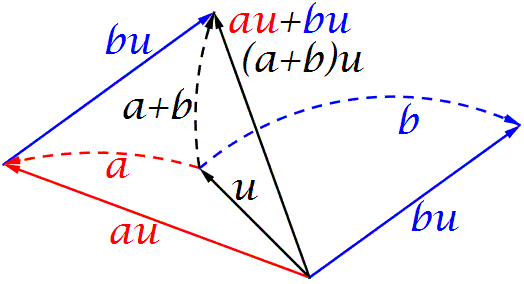
\includegraphics[width=0.5\textwidth]{imagenes/imagenes01/T01IM01.png}
		%\caption{Los dos problemas clásicos del cálculo: trazado de tangentes y áreas bajo curvas.}
	%\end{figure}
		
%varios párrafos encuadrados - explicaciones ad hoc
%\centering{
%\fbox{
%\parbox{0.95\textwidth}{
%varios
%
%$parrafos
%
%dentro
%}
%}
%}
% \justify


%\rotatebox{180}{\leftline{\textcolor{gris}{tararí}}}.